\documentclass{article}

\usepackage{amsthm}
\usepackage{amsfonts}
\usepackage{amsmath}
\usepackage{amssymb}
\usepackage{fullpage}
\usepackage[usenames]{color}
\usepackage{hyperref}
  \hypersetup{
    colorlinks = true,
    urlcolor = blue,       % color of external links using \href
    linkcolor= blue,       % color of internal links 
    citecolor= blue,       % color of links to bibliography
    filecolor= blue,        % color of file links
    }

\usepackage{listings}
\usepackage{graphicx}
\graphicspath{ {./Report Images/} }

\definecolor{dkgreen}{rgb}{0,0.6,0}
\definecolor{gray}{rgb}{0.5,0.5,0.5}
\definecolor{mauve}{rgb}{0.58,0,0.82}

\lstset{frame=tb,
  language=haskell,
  aboveskip=3mm,
  belowskip=3mm,
  showstringspaces=false,
  columns=flexible,
  basicstyle={\small\ttfamily},
  numbers=none,
  numberstyle=\tiny\color{gray},
  keywordstyle=\color{blue},
  commentstyle=\color{dkgreen},
  stringstyle=\color{mauve},
  breaklines=true,
  breakatwhitespace=true,
  tabsize=3
}

\theoremstyle{theorem} 
   \newtheorem{theorem}{Theorem}[section]
   \newtheorem{corollary}[theorem]{Corollary}
   \newtheorem{lemma}[theorem]{Lemma}
   \newtheorem{proposition}[theorem]{Proposition}
\theoremstyle{definition}
   \newtheorem{definition}[theorem]{Definition}
   \newtheorem{example}[theorem]{Example}
\theoremstyle{remark}    
  \newtheorem{remark}[theorem]{Remark}


\title{CPSC-406 Report}
\author{Marc Nathaniel Domingo  \\ Chapman University}

\date{\today}

\begin{document}

\maketitle

\begin{abstract}
The purpose of this course is to understand how the Theory of Algorithms coincide with the application of functions and algorithms in Software Engineering. In particular, this course places an emphasis on the concepts of Automata, Logic, and Concurrency in regard to algorithms in our eventual application of these topics to a final project. 
\end{abstract}

\tableofcontents

\section{Introduction}\label{intro}
\subsection{Week 1} During this week, the overall outline and "roadmap" of topics and project deadlines were covered during class, as well as an introduction to the concept of Definitive Finite Automata (DFA).
\subsection{Week 2} Lectures covered Definitive Finite Automata (DFA) and Non-Definitive Finite Automata (NFA) in more detail, as well as how to convert NFA to DFA.
\subsection{Week 3} During this week, the lectures covered the concepts of querying a database, as well as algorithms for Unification and Resolution.
\subsection{Week 4} During this week, lectures covered the concept of Distributed Hash Tables (DHT) in the application of Decentralized Systems.
\section{Homework}\label{homework}

This section contains solutions to homework. 

\subsection{Week 2}
The objective of this week's homework is to convert a given NFA to a DFA by hand.
\\ 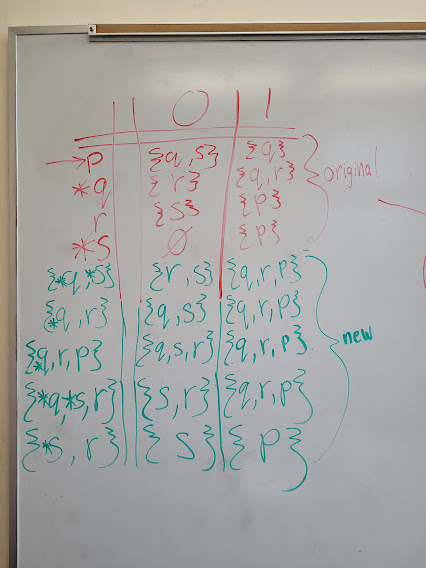
\includegraphics[width=15cm, height=8cm]{Report Images/HW2_1.jpg}
\\ 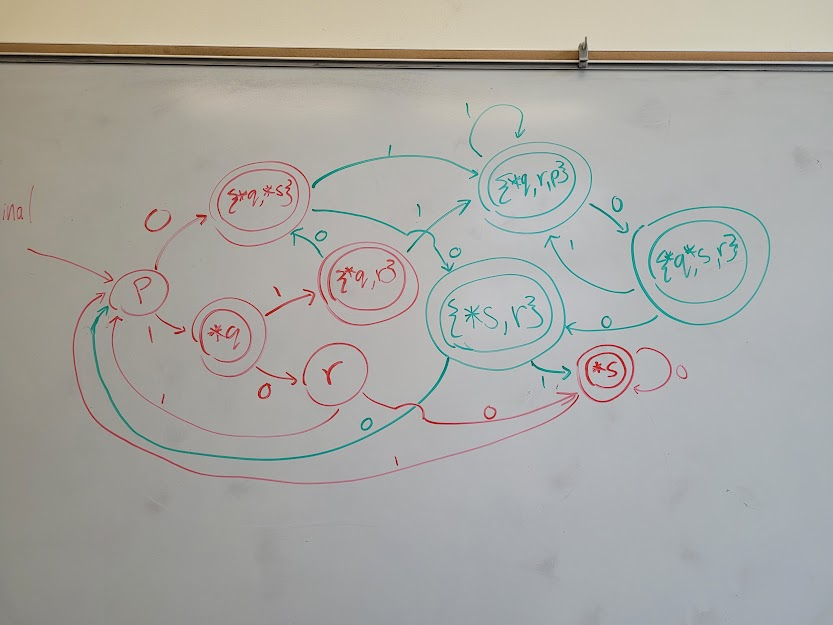
\includegraphics[width=15cm, height=8cm]{Report Images/HW2_2.jpg}
\subsection{Week 3}
The objective of this week's homework is to solve Unification Algorithm problems in addition to practicing drawing an SLD-tree solution to a program given a particular input.
\\ 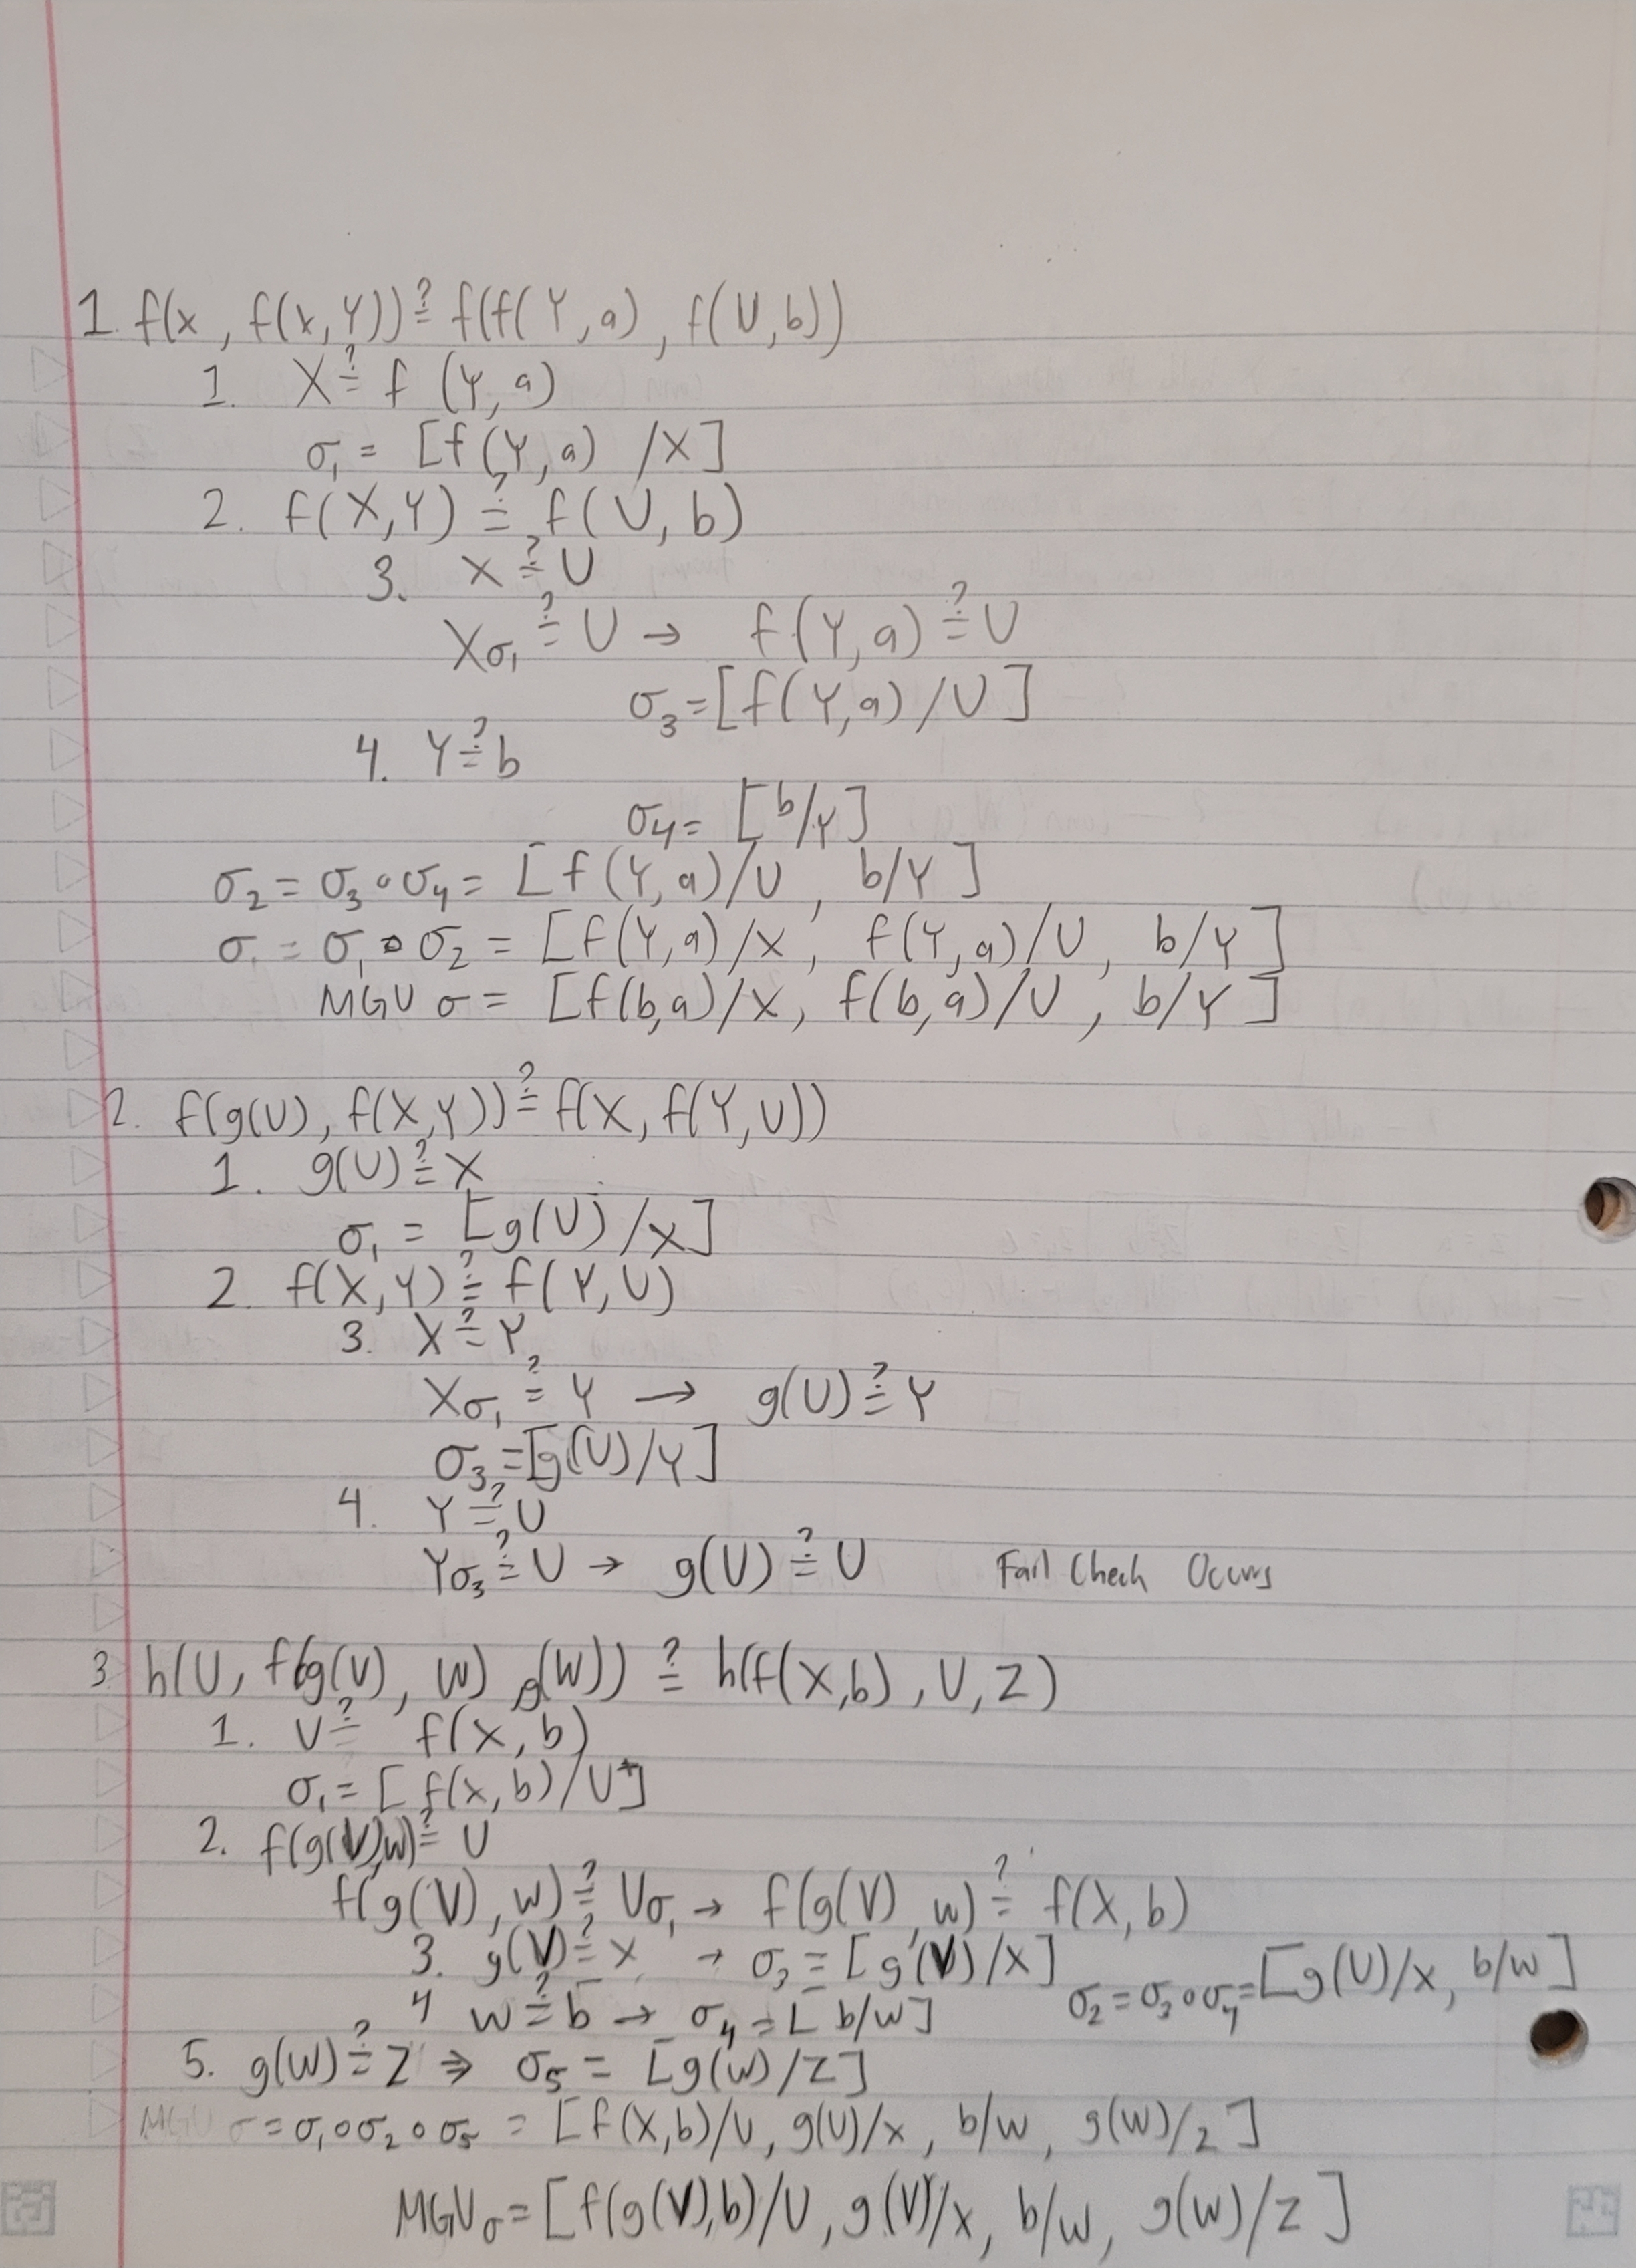
\includegraphics[width=18cm, height=20cm]{Report Images/HW3_1.jpg}
\\ 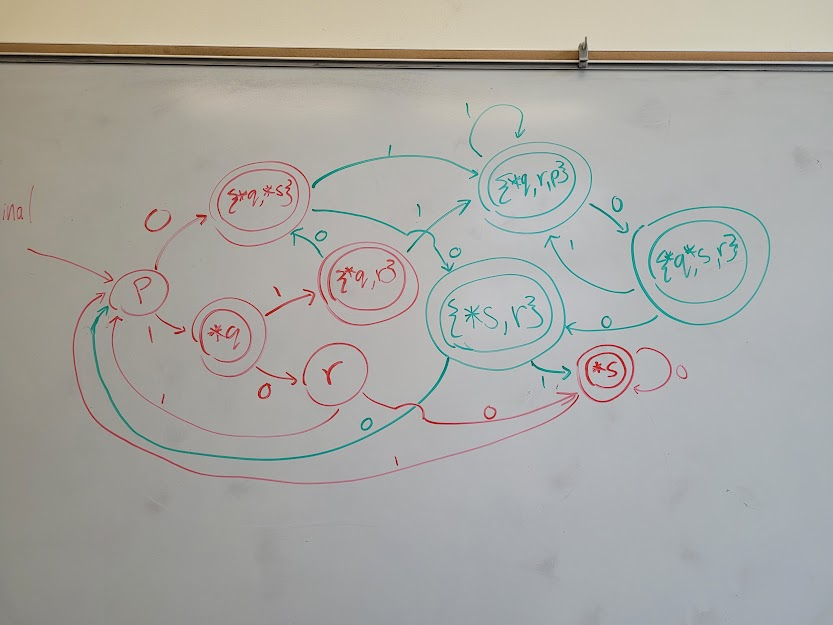
\includegraphics[width=18cm, height=20cm]{Report Images/HW3_2.jpg}
\section{Paper}

...

\section{Conclusions}\label{conclusions}

(approx 400 words) A critical reflection on the content of the course. Step back from the technical details. How does the course fit into the wider world of software engineering? What did you find most interesting or useful? What improvements would you suggest?

\begin{thebibliography}{99}
\bibitem[ALG]{Alg} \href{https://github.com/alexhkurz/algorithm-analysis-2023}{Algorithm Analysis}, Chapman University, 2023.
\end{thebibliography}

\end{document}